\begin{figure}[!ht]
\centering
\subfloat[L1 regularization]{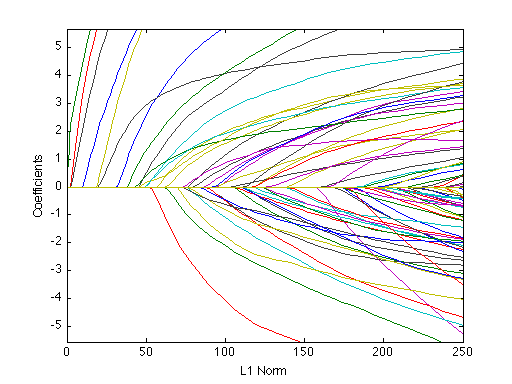
\includegraphics[width=.5\textwidth]{../images/lassoCoeffCurve.png}}
\subfloat[L2 regularization]{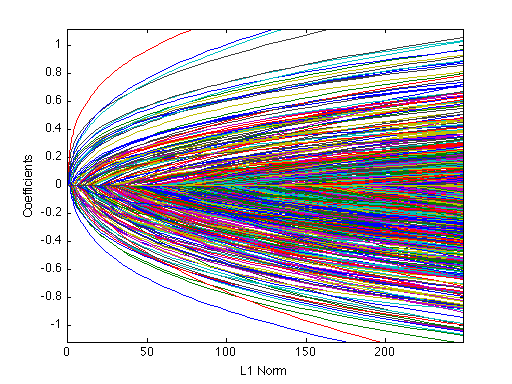
\includegraphics[width=.5\textwidth]{../images/ridgeCoeffCurve.png}}
\caption{Coefficient Paths for Regularized Logistic Regression}
%\label{fig:Coeff_paths}
\end{figure}


\begin{center}
\begin{figure}[!ht]
\centering
\subfloat[Unsorted]{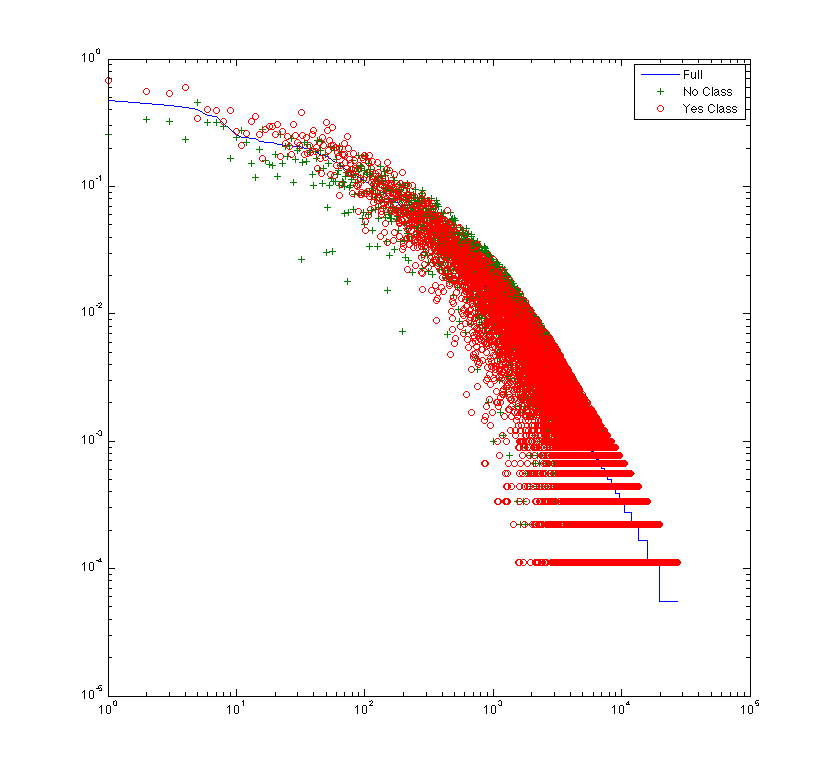
\includegraphics[width=.5\textwidth]{../images/zipfRankedFull.png}}
\subfloat[Sorted]{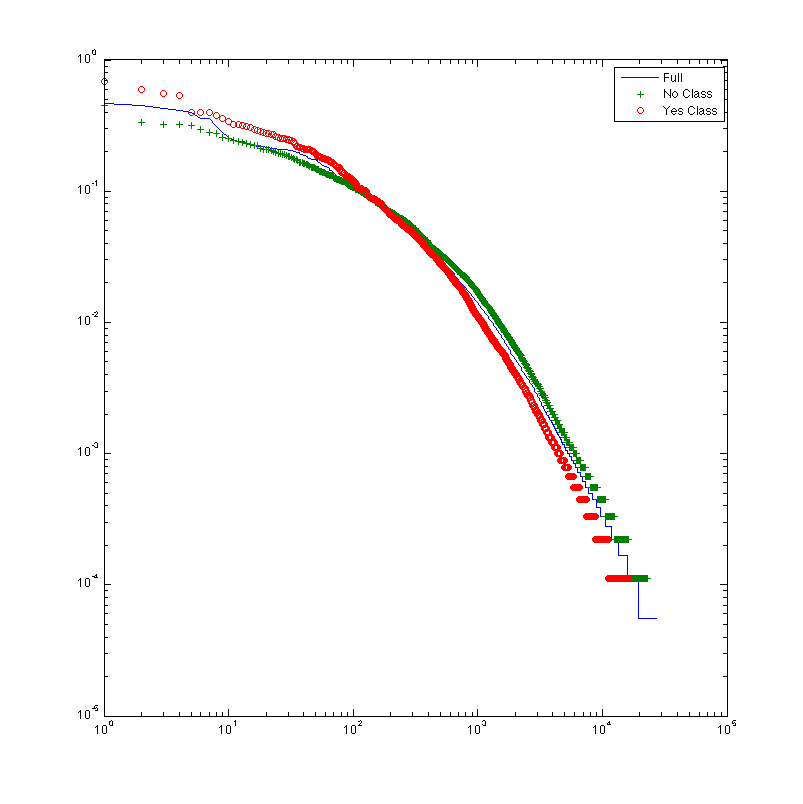
\includegraphics[width=.5\textwidth]{../images/zipfAllSorted.png}}
\caption{Frequency Vs. Rank in full data, target, and other classes}
\label{fig:largecompare}
\end{figure}
\end{center}

\begin{center}
\begin{figure}[!ht]
\centering
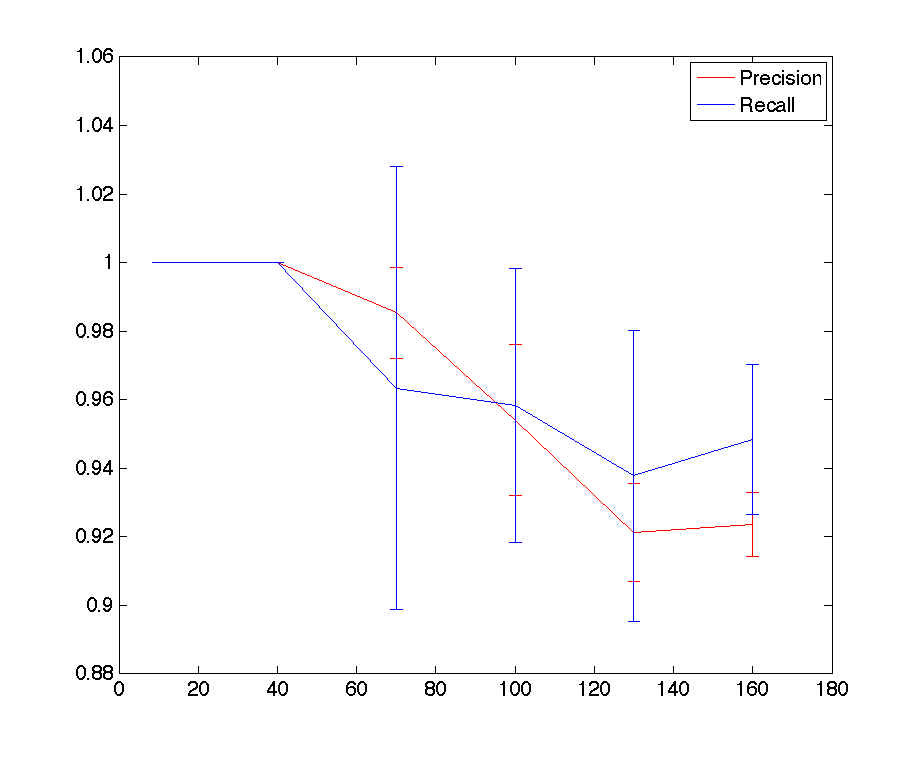
\includegraphics[width=.7\textwidth]{../images/precisionrecallExpansion.png}
\caption{Precision and Recall vs. Number of features selected using LASSO.}
\label{fig:prec recall}
\end{figure}
\end{center}

\begin{center}
\begin{figure}[!ht]
\centering
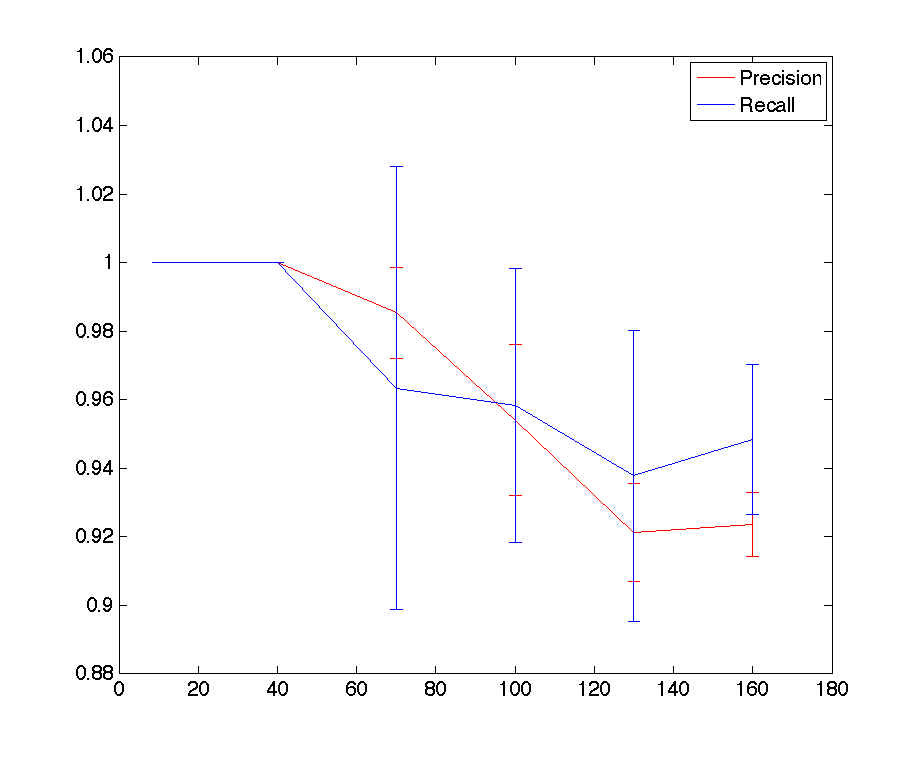
\includegraphics[width=.7\textwidth]{../images/precisionrecallExpansion.png}
\caption{Precision and Recall vs. Number of features selected using LASSO.}
\label{fig:prec recall}
\end{figure}
\end{center}

\begin{tabular}{cccccccccccc}
\hline
Mean&Mean STD&Native Mean&Native STD&Mean Benefit&Benefit STD
\\
\hline
0.9272&0.0099&0.9256&0.0123&-0.0016&0.0069
\end{tabular}


\begin{tabular}{cccccccccccc}
\hline
Precision Mean&Precision STD&Recall Mean&Recall STD
\\
\hline
.7570&0.2913&0.9456&0.1662
\end{tabular}


\begin{tabular}{cccccccccccc}
\hline
Mean Redundant At&Redundant At STD\\
\hline
72.5000&9.6982
\end{tabular}
